\chapter{Determinarea diametrului la butuc}\label{chapter:butuc}

Notații:
\begin{itemize}
    \item D $[m]$ - diametru
    \item R $[m]$ - rază
\end{itemize}

\

\noindent
Indici:
\begin{itemize}
    \item p - periferie
    \item b - butuc
    \item s - stagnare
    \item m - mijloc
\end{itemize}

\

Pentru a calcula diametrul la butuc $D_b$ folosim teoria dezvoltată la Timișoara de Susan-Resiga și exemplificată în \cite{susanhub}, care ne permite calculul teoretic al razei de stagnare fără a mai fi necesar un proces iterativ empiric până la obținerea unei valori care elimină riscul desprinderilor de pe butuc.

Pentru o rotație cu circulație constantă și o presiune totală constantă în conductă a fost dezvoltată în lucrarea \cite{susanhub} o ecuație algebrică pentru $x$ (definit ca $\big(R_s/R_p\big)^2$), dedusa cu ajutorul parametrului $\sigma$ și de unde putem obține o ecuație polinomială de gradul 3 în forma clasică:

\begin{equation}
\frac{\sigma^2}{x^2} - \frac{2}{(1-x^3)} = 0 \Rightarrow x^3 \sigma^2 + 2x^2 - \sigma^2 = 0
\end{equation}

Începem calculul parametrul (adimensional) de intensitate a rotației $\sigma$. Conform ecuației fundamentale a turbomașinilor (ecuația lui Euler) avem viteza tangențială la periferie:

\begin{equation}
gH=UV_{up}, \text{ sau } gH=\frac{\pi n}{30} R_{p} V_{up} \Rightarrow V_{up}=\frac{30gH}{\pi n R_{p}}
\end{equation}

Viteza axială medie (debitantă) prin conductă este:

\begin{equation}
V_{ad}=\frac{Q}{\pi R_{p}^2}
\end{equation}

În ambele ecuații, (3.2) și (3.3) raza conductei este practic raza de la periferie a turbinei. Ca rezultat, parametrul (adimensional) de intensitate a rotației este:

\begin{equation}
\sigma \equiv \frac{V_{up}}{V_{ad}} = 30 \frac{g H R_{p}}{n Q} = 30 \frac{9.81 \cdot 24 \cdot 0.110}{1500 \cdot 0.07} = 7.4
\end{equation}



Din (3.4) putem calcula raza de stagnare $R_{s}$ folosind metoda dezvoltată de Lebedev \cite{lebedev1991formulae} de rezolvare a ecuațiilor polinomiale de gradul 3 cu programul de calcul în Fortan de la anexa A.2.1. și obținem o valoare pentru $x$.

\begin{equation}
x = 0.73
\end{equation}

În regiunea (necunoscută) stagnantă $R_{s}$, se indică raportul de rază de stagnare față de raza la periferie, totul la pătrat, de unde putem obține raza de stagnare:

\begin{equation}
\text{Definim } x \equiv \bigg(\frac{R_{s}}{R_{p}}\bigg)^2 \Rightarrow R_{s} = \sqrt{x} \cdot R_{p} \Rightarrow \sqrt{0.73} \cdot 0.22 = 0.094\si{m}
\end{equation}

\begin{figure}[h!]
	\centering
	\includegraphics[scale=0.5]{figures/radius_stag-sigma.eps}
	\caption{Raportul dintre raza regiunii stagnante și raza țevii față de intensitatea rotației, pentru o rotație cu circulație constantă și o presiune totală constantă \cite{susanhub}}
	\label{Raportul dintre raza regiunii stagnante și raza țevii față de intensitatea rotației}
\end{figure}

În figura 3.1 putem observa corelația dintre intensitatea rotației pe abscise și raportul dintre raza de stagnare și raza la periferie a turbinei pe ordonata.

\begin{figure}[h!]
	\centering
	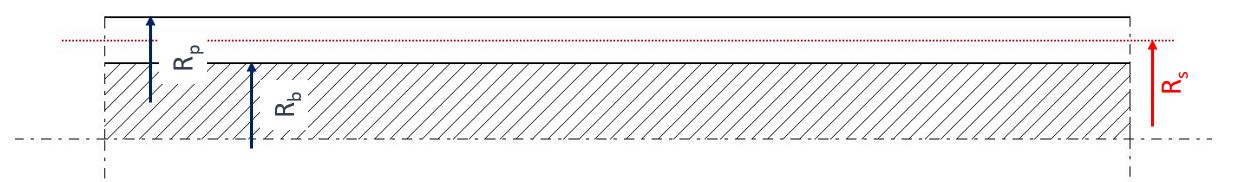
\includegraphics[scale=0.5]{figures/radii.jpg}
	\caption{Reprezentarea grafică a razelor din conducta în secțiune \cite{susanhub}}
	\label{Reprezentarea grafică a razelor din conducta în secțiune}
\end{figure}

După cum se poate observa în figura 3.2, la o valoare a razei de butuc egală sau mai mare decât raza de stagnare, înlăturam riscurile conform teoriei enunțate inițial. Astfel se alege pentru raza la butuc aceeași valoare ca și a razei de stagnare și anume $0.094\si{m}$.

\begin{equation}
R_b \geq R_s = 0.094\si{m}
\end{equation}

\clearpage